% @MOVE THIS

%% PIRMINIS SIGNALO APDOROJIMAS

\begin{cfigure}
  \centering
  \caption{Duomenų nuskaitymo funkcija iš tekstinės duomenų bylos}
  \label{code:read_data}
  \lstinputlisting{sources/read_data.m}
\end{cfigure}

Pirmoji funkcija, priklausanti pirminio signalo apdorojimo programai yra $read\_data$. Funkcijos kodas pateikiamas \ref{code:read_data} pav. Funkcijai užtenka nurodyti tik norimos nuskaityti bylos pavadinimą, kaip pavyzdžiui ``SiPt30\_01.txt'' ir funkcija gražins kairės kojos duomenis. Duomenų analizėje naudojami tik vienos kojos duomenis, kadangi dešinės ir kairės kojos duomenys yra stipriai koreliuoti \cite{16053531}, todėl nėra prasmės naudoti dviejų kojų duomenų. Pasirinkus tokį sprendimą taip pat yra sumažinamas skaičiavimų skaičius programoje. Duomenų bazės direktorija nurodyti kintamojo vietoje yra taip pat svarbus aspektas, kadangi pakitus duomenų bazės vietai, užteks tik pakeisti vieną kintamąjį, o ne visą kodą, nors kodas ir nėra ilgas. Matlab funkcija $dlmread$ gražina duomenis masyvo pavidalu, kur stulpelis nurodo įvade aptartus duomenis, o eilutė nurodo duomenų vertes tam tikru laiko momentu.

\begin{cfigure}
  \centering
  \caption{Slankiojančio lango algoritmo pritaikymas}
  \label{code:sliding_window}
  \lstinputlisting{sources/split_data.m}
\end{cfigure}

Sekantis žingsnis, po duomenų nuskaitymo, yra jų pirminis apdorojimas. Nagrinėjimas pradėtas nuo slankiojančio lango metodo. Programos kodas pateikiamas \ref{code:sliding_window} pav. Funkcijos įvestyje pateikiamas nagrinėjamas signalas, slankiojamo lango ilgis ir slankiojamo lango perdanga. Slankiojamo lango perdanga nurodo reikšmių arba laiko verčių kiekį, kurį algoritmas pašalina iš spartinančiosios atminties, laukdamas naujų verčių langui užpildyti. Pavyzdžiui, jeigu lango ilgis yra $4$ signalo verčių, o perdanga -- $2$ signalo vertės, vadinasi, kai algoritmas užpildys langą $4$ signalo vertėm, esamą langą jis perduos į išėjimo spartinančiąją atmintį, paskutines dvi vertes ištrins iš spartinančiosios atminties ir iš naujo lauks naujų dviejų reikšmių langui pilnai užpildyti.

Funkcija yra tiek lanksti, kad nėra svarbu kokio tipo duomenys yra pateikiami -- ar tai konkretaus signalo vertės ar iš ankščiau pritaikyto slankiojančio lango algoritmo išskirti signalo požymiai, kurie panaudoti formuojant naują signalą. Tokia funkcijos savybė labai naudinga tolimesniame darbe.

\begin{cfigure}
  \centering
  \caption{Signalo filtravimas dviem Butterworth filtrais}
  \label{code:filter}
  \begin{lstlisting}
    [B,A] = butter(9, 1/50, 'high');
    [BB,AA] = butter(9, 40/50, 'low');
    output = filter(BB, AA, filter(B, A, input));
  \end{lstlisting}
\end{cfigure}

Sekanti programos dalis atlieka paprastą signalo filtravimą su dvejais $Butterworth$ skaitmeniniais filtrais. Pirmasis, aukštų dažnių filtras, skirtas pašalinti signalo nuolatinei komponentei. Antras, žemų dažnių filtras, skirtas pašalinti aukšto dažnio triukšmą, kuris neneša visiškai jokios naudingos informacijos. Filtras įgyvendinamas labai paprastai. Kodo pavyzdys pateikiamas \ref{code:filter} pav. Abiejų filtrų eilė yra 9-ta, žemų dažnių filtro ribinis dažnis parinktas $40$ Hz. Duomenys diskretizuojami $100$ Hz dažniu, vadinasi didžiausias galimas signalo dažnis yra $50$ Hz. Didžiausias žmogaus generuojamas dažnis ėjimo metu, remiantis šaltiniu, yra $20$ Hz. Užtikrintumui parinktas $40$ Hz dažnis. Nuolatinė dedamoji pašalinama su aukšto dažnio filtru, kurio ribinis dažnis yra $1$ Hz. Nuolatinė dedamoji neneša jokios informacijos apie eisena, kadangi ji tiktais nurodo naudojamų jutiklių jautrumą.

\begin{cfigure}
  \centering
  \caption{Kontakto su žeme signalo išskyrimo programos kodo fragmentas}
  \label{code:signal_extraction}
  \lstinputlisting{sources/extract_signal.m}
\end{cfigure}

Toliau seka, priklausomai nuo pasirinkto pirminio signalų apdorojimo būdo, signalo išskyrimas pagal fizinę veiklą. Dominančios signalo būsenos yra, kai subjekto koja turi kontaktą su žeme ir nurodytas subjektas neturi kontakto su žeme. Kontakto su žeme signalo išskyrimui programos kodas yra pateikiamas \ref{code:signal_extraction} pav.

Pirmiausiai, ``Pt\_t'' kintamojo struktūroje yra saugoma kairės kojos Parkinsono liga sergančių subjektų duomenys. Kiekvienas signalas yra priskiriamas prie $signal$ kintamojo, su kuriuo toliau yra tęsiamas apdorojimo procesas. Jeigu signalas nėra lygus nuliui, tuomet jis įdedamas į laikinąją atmintį. Taip signalas yra tikrinamas iki tol, kol signalas tampa lygus nuliui ir tęsiamas tolimesnis apdorojimas. Apdorojimas susideda iš signalo ilgio patikros. Jeigu signalas yra trumpesnis už 10 verčių, arba turint omenyje, kad signalas diskretizuojamas $100$ Hz, tai $0,1$ s, vadinasi, signalas yra tiesiog aukšto dažnio triukšmas arba blogas pavyzdys ir signalas yra atmetamas. Jeigu signalas yra ilgesnis už 200 verčių ($2$ s), vadinasi, duomenų rinkimo metu įvyko klaida ir koja per tokį laiką nebuvo pakelta. Tokia klaida gali būti sukelta, kuomet subjektas ne eina, o stovi ant dviejų kojų arba tik ant kairės kojos. Jeigu visi kriterijai patenkinami, signalas yra priimamas ir kraunamas į laikinąją atmintį, pavadinimu ``$data.Pt$''. Signalas, kuriuo metu koja neliečia žemės, yra randamas kartu su ankščiau išnagrinėtu metu. Algoritmas patikrina kiek praėjo laiko (arba kiek verčių yra priskaičiuota) nuo paskutinio užskaityto kojos ant žemės signalo ir įrašo tą signalą į laikiną atmintį, jeigu po praeito signalo nepraėjo mažiau negu 50 verčių arba $0,5$ s ir nedaugiau nei 200 verčių arba $2$ s. Kojos signalas yra pateiktas \ref{fig:stance_phase} pav.

\begin{figure}[!t]
  \centering
  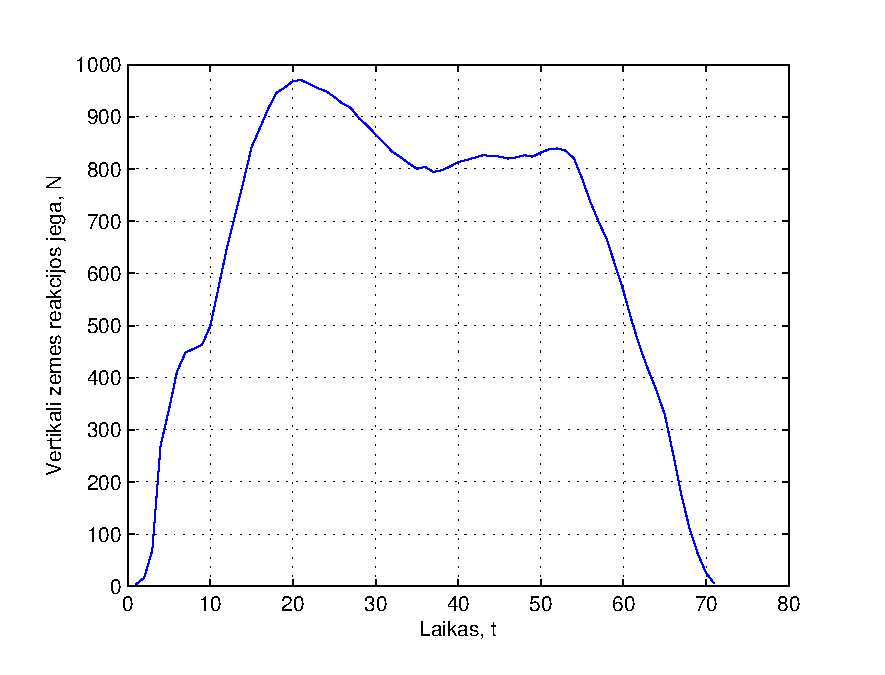
\includegraphics[width=300px]{figures/09_sample_stance_phase.eps}
  \caption{Susilietimo su žeme signalas}
  \label{fig:stance_phase}
\end{figure}

\begin{figure}[!t]
  \centering
 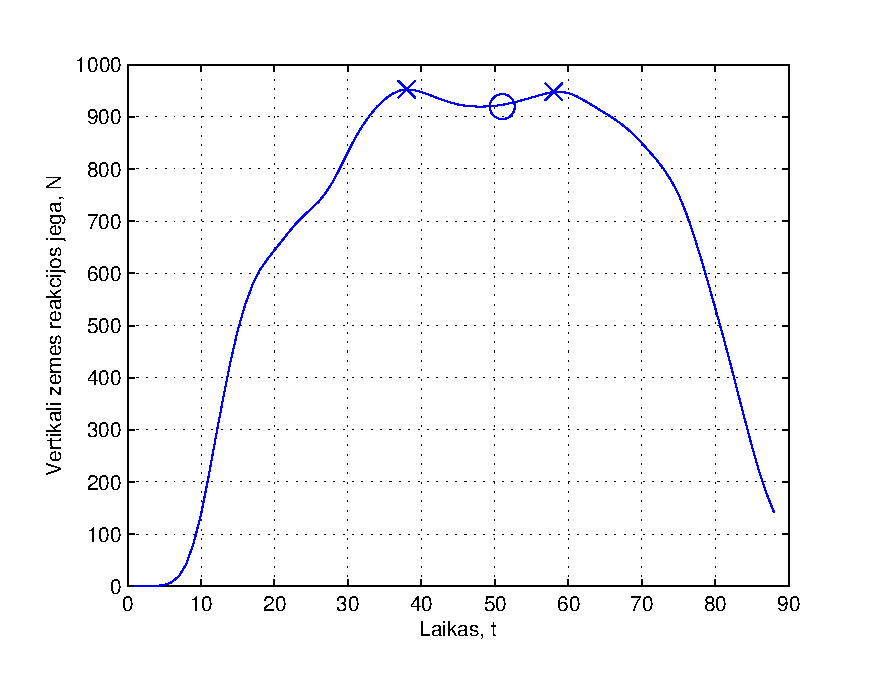
\includegraphics[width=300px]{figures/10_global_max_local_min.eps}
  \caption{Dviejų globalių maksimumų ir vieno lokalaus minimumo radimas signale}
  \label{fig:min_max}
\end{figure}


% TODO: ref

Dar vienas pirminio signalo apdorojimas, kuris panaudotas tiriant galima bendrą erdvę -- kojos prisilietimo prie žemės signalo dviejų globalių maksimumų ir vieno lokalaus minimumo paieška \cite{6151536}. Algoritmo rezultatas yra pateiktas \ref{fig:min_max} pav. Kryžiais pažymėtos globalaus maksimumo vietos, apskritimu pažymėta lokalaus minimumo signalo vieta. Išanalizavus daugumos subjektų žingsnio signalus, padaryta išvada, kad kiekviename žmogaus žingsnyje egzistuoja du maksimumai. Vienas maksimumas randamas, kai subjektas yra visiškai atsirėmęs galine pėdos dalimi į žemę, antras maksimumas randamas, kai subjektas visiškai atsiremia priekinę pėdos dalimi. Tarp šių dviejų maksimumų yra pereinamasis laikotarpis, kuris yra signalo lokalus minimumas. Priežastis, dėl kurios algoritmas įgyvendintas, yra vienas darbas \cite{6151536}, kuriame pasiūlyta naudotis būtent tokiais požymiais atpažinti Parkinsono liga sergančius subjektus nuo nesergančių subjektų. Pačio algoritmo kodo dalis yra pateikta \ref{code:min_max} pav.

\begin{cfigure}[!t]
  \centering
  \caption{Dviejų globalių maksimumų ir vieno lokalaus minimumo radimo algoritmo fragmentas}
  \label{code:min_max}
  \lstinputlisting{sources/min_max.m}
\end{cfigure}

Programos kodas kaupia gaunamą signalą į laikinąją atmintį ir tikrina ar signalas pakito per užduotą dydį $\delta$. Delta nurodo kiek signalas turi pakisti, kad algoritmas nustatytų signalo mažėjimo pradžią. Tokio tikrinimo priežastis yra signalo kilimo sumažėjimas prieš globalų maksimumą. Kai kuriuose pavyzdžiuose buvo net pastebėtas signalo mažėjimas. Dėl šios priežasties buvo įvesta pokyčio tikrinimo metodas.